\documentclass{beamer}
\usepackage[utf8x]{inputenc}
\usepackage[czech]{babel}
\usepackage{booktabs}
\usepackage{listings}

\usetheme[pageofpages=of,% String used between the current page and the
                         % total page count.
          bullet=circle,% Use circles instead of squares for bullets.
          titleline=true,% Show a line below the frame title.
	  titlepagelogo=opensuse,
          alternativetitlepage=true,% Use the fancy title page.
          ]{Torino}

\setbeamerfont{title}{series=\bfseries,size=\LARGE}
\author{Tom\'{a}\v{s} Chv\'{a}tal\newline {\small SUSE Packagers team}}
\title{Buildsystems and what the heck for we actually use the autotools}
\date{2013/07/19}

\AtBeginSection[]
{
	\setbeamercolor{background canvas}{bg=chameleongreen3}
	\begin{frame}[plain]
		\begin{center}\begin{huge}\textcolor{white}{\secname}\end{huge}\end{center}
	\end{frame}
	\setbeamercolor{background canvas}{bg=}
}

\AtBeginSubsection[]
{
	\setbeamercolor{background canvas}{bg=chameleongreen3}
	\begin{frame}[plain]
		\begin{center}\begin{huge}\textcolor{white}{\subsecname}\end{huge}\end{center}
	\end{frame}
	\setbeamercolor{background canvas}{bg=}
}

\begin{document}

\begin{frame}[t,plain]
\titlepage
\end{frame}

\section{Introduction}

\begin{frame}[t]{Who the hell is Tomáš Chvátal}
	\begin{itemize}
	\item SUSE Employee since 2011 - Team lead of packagers team
	\item Packager of Libreoffice and various other stuff for openSUSE
	\item openSUSE promoter and volunteer
	\item Gentoo developer since fall 2008
	\end{itemize}
\end{frame}

\section{Autotools process}

\begin{frame}{Complete autotools process}
	\begin{figure}
	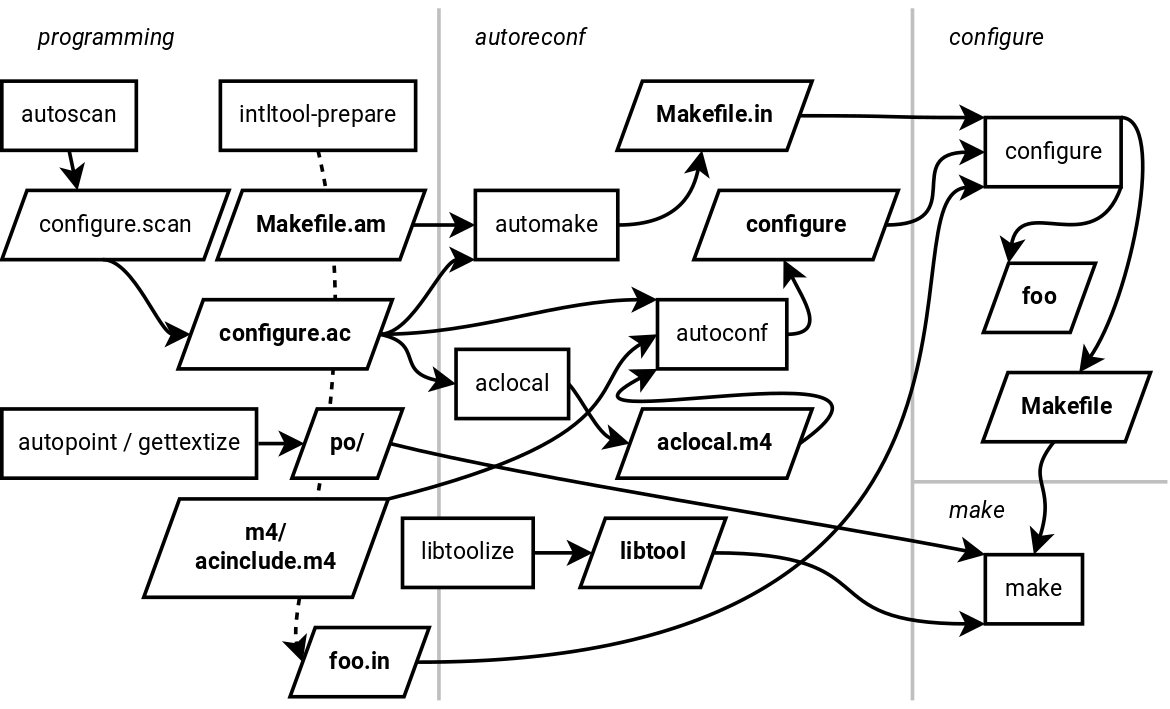
\includegraphics[width= 1.0\linewidth]{autotools.png}
	\end{figure}
\end{frame}

\begin{frame}{Simplified autotools process}
	\begin{figure}
	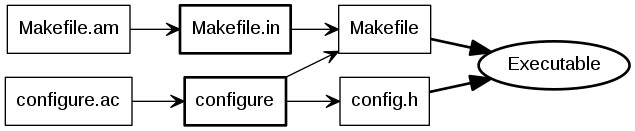
\includegraphics[width= 1.0\linewidth]{autotools_simple.png}
	\end{figure}
\end{frame}

\subsection{Libtool}

\begin{frame}{Libtool versioning}
	\begin{itemize}
	\item Start with version information of ‘0:0:0’ for each libtool library
	\item If the library source code has changed at all since the last update, then increment revision (‘c:r:a’ becomes ‘c:r+1:a’)
	\item If any interfaces have been added, removed, or changed since the last update, increment current, and set revision to 0
	\item If any interfaces have been added since the last public release, then increment age
	\item If any interfaces have been removed or changed since the last public release, then set age to 0
	\end{itemize}
\end{frame}

\begin{frame}[t]{configure.ac changes}
	\begin{small}
	\lstinputlisting{autoconflibtool.txt}
	\end{small}
\end{frame}

\begin{frame}[t]{Makefile.am changes}
	\begin{small}
	\lstinputlisting{automakelibtool.txt}
	\end{small}
\end{frame}

\section{Reading}

\begin{frame}{Reading}
	\begin{figure}
	
\includegraphics[width= 0.4\linewidth]{mythbuster.png}
	\end{figure}
\end{frame}

\section{Endnote}

\begin{frame}{Thanks}
	\begin{center}
	Thank you for your attention.
	\end{center}
\end{frame}

\end{document}

